\section{Hyperparameter selection}

\subsection{Hierarchical clustering}

The chosen hyperparameters for the Hierarchical clustering model are as follows:

\begin{itemize}
    \item \textbf{Method = Ward:} Because our data is numerical, and we want compact clusters the method choice is straight forward. Ward's method minimizes the total within cluster variance which results in compact and homogeneous clusters.
    
    \item \textbf{Metric = Euclidean:} Ward's method requires the use of the distance function Euclidean, when comparing alternative methods (average, complete, etc) with other distance functions we do not observe similarly effective cluster separations. Therefore strengthening our choice of Ward's method and Euclidean distance.
    \item \textbf{Number of clusters = 5:} The number of clusters is chosen by creating and analyzing a dendogram, where the number of clusters is determined by drawing a horizontal line at the top of the dendogram. The horizontal line is placed so the distances between horizontal lines above are big, indicating that each cluster is far apart from eachother. We also consider the silhouette score of different amonunt of clusters. We choose 5 clusters, but discussions with domain experts about our clustering results could lead to a different number of clusters. Silhouette score bar plot and dendogram can be seen in \autoref{fig:silhouette_agglomerative} and \autoref{fig:dendrogram} below:
\end{itemize}

\begin{figure}[H]
    \hspace*{\fill}
    \centering
    \begin{subfigure}[b]{0.45\textwidth}
        \centering
        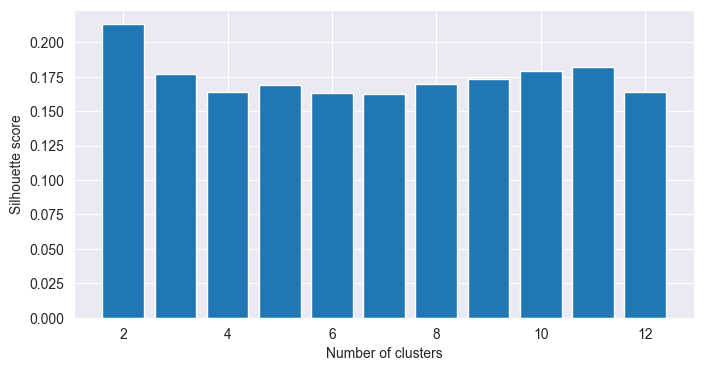
\includegraphics[width=1.0\textwidth]{src/figs/silhouette_agglomerative.png} 
        \caption{Silhouette scores for agglomerative clustering}\label{fig:silhouette_agglomerative}
    \end{subfigure}
    \hfill
    \begin{subfigure}[b]{0.45\textwidth}
        \centering
        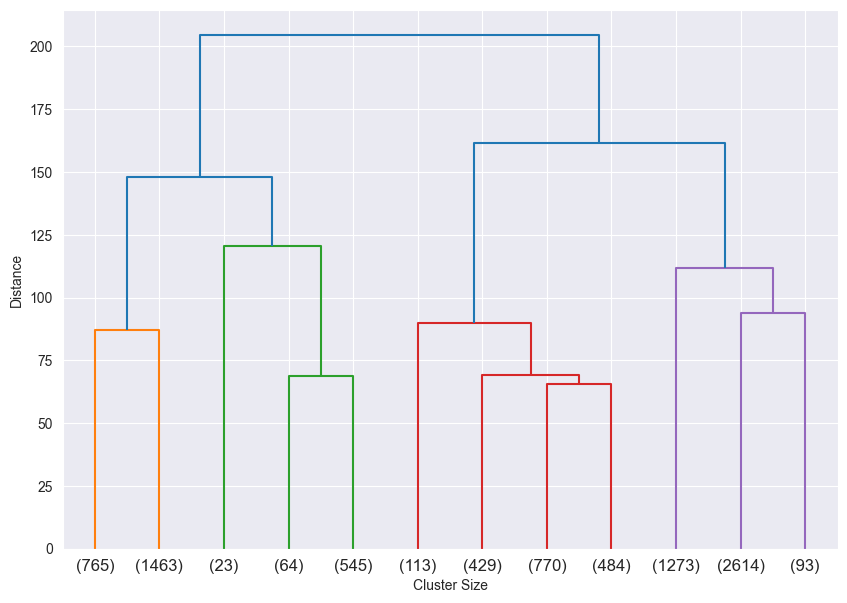
\includegraphics[width=1.0\textwidth]{src/figs/dendrogram.png} 
        \caption{Dendrogram}\label{fig:dendrogram}
    \end{subfigure}\label{fig:silhouette_dendrogram}
    \caption{Hierarchical clustering hyperparameter selection}\label{fig:hyperparameters_hierarchical}
    \hspace*{\fill}
\end{figure}



\subsection{DBSCAN}

The chosen hyperparameters for the DBSCAN model are as follows:

\begin{itemize}
    \item \textbf{Min samples = 17:} A rule of thumb for choosing min\_samples is to set it to be the number of features in the dataset plus one. In our case, we have $16$ features, so we set min\_samples to $17$.
    \item \textbf{Epsilon = 0.3:} The epsilon value is chosen by first calculating the distance of each point to it's $17$-th nearest neighbor. Choosing $17$-th nearest in our case because that is our min\_samples. We then plot a histogram to find a knee to define an appropriate epsilon value. The histogram can be seen in \autoref{fig:epsilon_histogram} below. The knee seems to be found at somewhere between $0.25$ and $0.35$. To chose a good value between these two, we also look at the silhouette score for the different epsilon values, found in \autoref{fig:silhouette_epsilon}. We choose $0.3$ as our epsilon value.
\end{itemize}

\begin{figure}[H]
    \hspace*{\fill}
    \centering
    \begin{subfigure}[b]{0.45\textwidth}
        \centering
        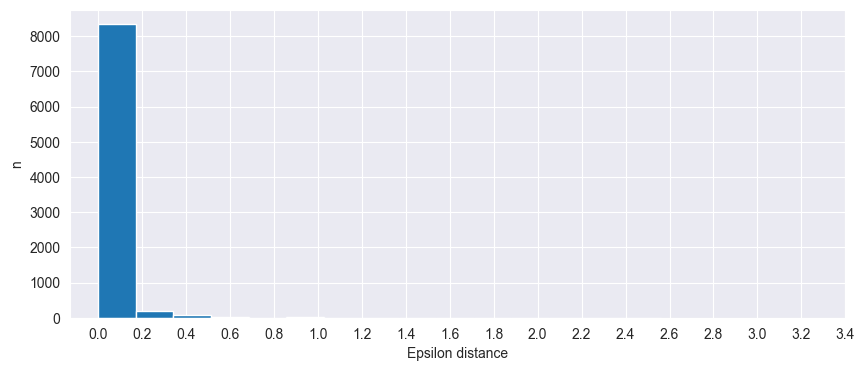
\includegraphics[width=1.0\textwidth]{src/figs/epsilon_histogram.png} 
        \caption{Epsilon value histogram}\label{fig:epsilon_histogram}
    \end{subfigure}
    \hfill
    \begin{subfigure}[b]{0.45\textwidth}
        \centering
        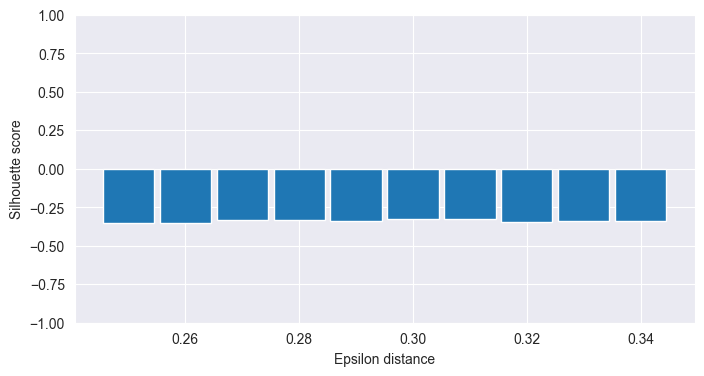
\includegraphics[width=1.0\textwidth]{src/figs/silhouette_epsilon.png} 
        \caption{Silhouette scores for different epsilon values}\label{fig:silhouette_epsilon}
    \end{subfigure}
    \caption{Epsilon hyperparameter selection}\label{fig:hyperparameters_dbscan}
    \hspace*{\fill}
\end{figure}
